% !TEX root = sum1.tex
\section{Problem Description}
In this section, to incorporate the social distancing into seat planning, we first give the description of the seat planning problem with social distancing. Then we introduce the dynamic seat assignment problem with social distancing.

% dynamic seat assignment problem, which is suitable for commercial use in cinemas and concerts.

\subsection{Seat Planning Problem with Social Distancing}\label{dynamic_demand}
We consider a layout comprising $N$ rows, with each row containing $L_j^0$ seats, where $j \in \mathcal{N} \coloneqq \{1,2, \ldots, N\}$. The seating arrangement is used to accommodate various groups, where each group consists of no more than $M$ individuals. There are $M$ distinct group types, denoted by group type $i$, where each group type consists of $i$ people. The set of all group types is denoted by $\mathcal{M} = {1, 2, \ldots, M}$. The demand for each group type is represented by a demand vector $\mathbf{d} = (d_1, d_2, \ldots, d_M)^{\intercal}$, where $d_i$ represents the number of group type $i$.

In order to comply with the social distancing requirements, individuals from the same group must sit together, while maintaining a distance from other groups. Let $\delta$ denote the social distancing, which could entail leaving one or more empty seats. Specifically, each group must ensure the empty seat(s) with the adjacent group(s).

% Importantly, the seating arrangement of different rows does not affect each other, meaning that individuals from one group can be seated directly behind individuals from another group.

To model the social distancing requirements into the seat planning process, we add the parameter, $\delta$, to the original group sizes, resulting in the new size of group type $i$ being denoted as $n_i = i + \delta$, where $i \in \mathcal{M}$. Accordingly, the length of each row is also adjusted to accommodate the adjusted group sizes. Consequently, $L_j = L_j^{0} + \delta$ represents the length of row $j$, where $L_j^{0}$ indicates the number of seats in row $j$. By incorporating the additional seat(s) and designating certain seat(s) for social distancing, we can integrate social distancing measures into the seat planning problem.

% the seat layout is modified by adding $\delta$ to the length of each row. 
% Consequently, the new size of group type $i$ is denoted as $n_i = i + \delta$. 


Let $x_{ij}$ represent the number of group type $i$ planned in row $j$. The deterministic seat planning problem is formulated below, with the objective of maximizing the number of people accommodated.

\begin{equation}\label{deter_upper}
  \begin{aligned}
  \max \quad & \sum_{i=1}^{M}  \sum_{j= 1}^{N} (n_i- \delta) x_{ij} \\
  \text {s.t.} \quad & \sum_{j= 1}^{N} x_{ij} \leq d_{i}, \quad i \in \mathcal{M}, \\
  & \sum_{i=1}^{M} n_{i} x_{ij} \leq L_j, j \in \mathcal{N}, \\
  & x_{ij} \in \mathbb{Z}_{+}, \quad i \in \mathcal{M}, j \in \mathcal{N}.
  \end{aligned}
\end{equation}

This seat planning problem can be regarded as a special case of the multiple knapsack problem. In this context, we define $X$ as the aggregate solution, where $X = (\sum_{j=1}^{N} x_{1j}, \ldots, \sum_{j=1}^{N} x_{Mj})$. Each element of $X$, $\sum_{j=1}^{N} x_{ij}$, represents the available supply of seats for group type $i$. In other words, $X$ captures the total number of seats that can be allocated to each group type by summing up the supplies across all rows. By considering the monotone ratio between the original group sizes and the adjusted group sizes, we can determine the supply corresponding to the optimal solution of the LP relaxation of Problem \eqref{deter_upper}, as demonstrated in Proposition \ref{sol_relax_deter}.

Although the problem size is small and the optimal solution can be easily obtained using a solver, it is still important to analyze the problem further to gain additional insights and understanding.
We introduce the term pattern to refer to the seat planning arrangement for a single row. A specific pattern can be represented by a vector $\bm{t} = (t_1, \ldots, t_M)$, where $t_i$ represents the number of group type $i$ in the row for $i = 1,\ldots, M$. This vector $\bm{t}$ must satisfy the condition $\sum_{i=1}^{M} t_i n_i \leq L$ and belong to the set of non-negative integer values, denoted as $\bm{t} \in \mathbb{Z}_{+}^{M}$.

In order to quantify the impact of each pattern, we introduce the concept of loss, which is the number of unoccupied seats. Mathematically, the loss is defined as $L- \delta - \sum_{i =1}^{M} i t_i$, where $L$ denotes the length of the row.

The loss provides a measure of the number of seats which cannot be taken due to the implementation of social distancing constraints. By examining the losses associated with different patterns, we can assess the effectiveness of various seat planning configurations with respect to accommodating the desired number of individuals while adhering to social distancing requirements.

\begin{definition}
Consider the length of the row is $L$, the social distancing is $\delta=1$ and a pattern $(t_1, \ldots, t_M)$.
We call the pattern $\bm{t}$ a full pattern if it satisfies the condition $\sum_{i=1}^{M} t_i n_i = L$. We call the pattern $\bm{t}$ a largest pattern if it belongs to $\arg\min_{\bm{t}} \{L - \delta - \sum_{i =1}^{M} i t_i\}$.

% minimizes the loss $L - \delta - \sum_{i =1}^{M} t_i \cdot i$ for all $\bm{t}$ that satisfy the constraint $\sum_{i=1}^{M} t_i n_i \leq L$. 

% This means that all available seats in the row are fully occupied by the groups. In other words, a largest pattern is one that accommodates the maximum number of individuals while minimizing the number of unoccupied seats, taking into account the social distancing requirement.

% If $\bm{t}$ minimizes the loss $L- \delta - \sum_{i =1}^{M} t_i \cdot i$ for all $t$ satisfying $\sum_{i=1}^{M} t_i n_i \leq L$, the corresponding pattern is defined as a largest pattern.
% The loss of the pattern $L- \delta - \sum_{i =1}^{M} t_i^{l} \cdot i$ is less than any other pattern. we call the pattern with the minimal loss as the largest patterns.

% Additionally, we refer to patterns that have no empty seats, except for those reserved for social distancing purposes, as full patterns.
\end{definition}

In many cases, the optimal solution for the seat planning problem tends to involve rows with either full patterns or the largest patterns. Distinguishing these patterns from other configurations can provide valuable insights into effective seat planning strategies that prioritize accommodating as many people as possible while adhering to social distancing guidelines.

When there is high demand for seats, it is advantageous to prioritize the largest patterns. These patterns allow for the accommodation of the largest number of individuals due to social distancing requirements. On the other hand, in scenarios with moderate demand, adopting the full pattern becomes more feasible. The full pattern maximizes seating capacity by utilizing all available seats, except those needed for social distancing measures.

By considering both the largest and full patterns, we can optimize seat planning configurations to efficiently accommodate a significant number of individuals while maintaining adherence to social distancing guidelines. 

% This approach allows for effective and efficient use of available seating capacity.

\begin{prop}\label{lem_pattern}
When given the length of a row, $L$, the social distancing, $\delta$, the adjusted size of the largest group allowed, $n_M$, the loss of the largest pattern is $\lfloor \frac{L}{n_M} \rfloor \delta - \delta + g(L - \lfloor \frac{L}{n_M} \rfloor n_M)$, where $g(r) = 0$ if $r > \delta$, and $g(r) = r$ if $r \leq \delta$.
\end{prop}

% the social distancing requirement is one seat. In this case, the new sizes of the groups would be 2, 3, 4, and 5, respectively.
\begin{example}
Consider the given values: $\delta = 1$, $L = 21$, and $M = 4$. In this case, we have $n_i = i + 1$ for $i \in {1, 2, 3, 4}$. The loss of the largest pattern can be calculated as $\lfloor \frac{21}{5} \rfloor - 1 + g(1) = 5$. The largest patterns are the following: $(1, 0, 1, 3)$, $(0, 1, 2, 2)$, $(0, 0, 0, 4)$, $(0, 0, 4, 1)$, and $(0, 2, 0, 3)$. 
\end{example}

% Additionally, the pattern $(1, 1, 4, 0)$ is a full pattern.
% Please note that the pattern sizes and specific patterns may vary depending on the values of $L$, $M$, and $n_i$.

Through this example, we observe that the largest pattern does not exclusively consist of large groups but can also include smaller groups. This highlights the importance of considering the various group sizes when generating the largest pattern. Another observation relates to the relationship between the largest patterns and full patterns. It is apparent that a full pattern may not necessarily be the largest pattern. For instance, consider the pattern $(1, 1, 4, 0)$, which is a full pattern as it utilizes all available seats. However, its loss value is 6, indicating that it is not the largest pattern. Conversely, a largest pattern may also not necessarily be a full pattern. Take the pattern $(0, 0, 0, 4)$ as an example. It is a largest pattern as it can accommodate the maximum number of individuals. However, it does not satisfy the requirement of fully utilizing all available seats since $4 \times 5 \neq 21$.


% We consider the social distancing of one empty seat throughout the rest of this paper, which is more practical and reasonable in the seat planning. However, our methods are still applicable to the social distancing of two or more seats.

% Next, we will analyze the impact of implementing social distancing on each row. We define seat planning as the arrangement of seats within a row, specifically, the number of different group types present in each row, as long as the sum of the sizes of all groups is no larger than the length of the row.  

Although the optimal solution to the seat planning problem is complex, the LP relaxation of problem \eqref{deter_upper} has a nice property.

\begin{prop}\label{sol_relax_deter}
In the LP relaxation of problem \eqref{deter_upper}, there exists an index $h$ such that the optimal solutions satisfy the following conditions:

\begin{itemize}
  \item For $i = 1,\ldots, h-1$, $x_{ij}^{*} = 0$ for all rows, indicating that no group type $i$ are assigned to any rows before index $h$.
  \item For $i = h+1,\ldots, M$, the optimal solution assigns $\sum_{j} x_{ij}^{*} = d_{i}$ group type $i$ to meet the demand for group type $i$.
  \item For $i = h$, the optimal solution assigns $\sum_{j} x_{ij}^{*} = \frac{L - \sum_{i = h+1}^{M} {d_i n_i}}{n_h}$ group type $h$ to the rows. This quantity is determined by the available supply, which is calculated as the remaining seats after accommodating the demands for group types $h+1$ to $M$, divided by the size of group type $h$, denoted as $n_h$.
\end{itemize}

Hence, the corresponding supply values can be summarized as follows: $X_h = \frac{L - \sum_{i = h+1}^{M} {d_i n_i}}{n_h}$, $X_{i} = d_{i}$ for $i = h+1,\ldots, M$, and $X_{i} = 0$ for $i = 1, \ldots, h-1$. These supply values represent the allocation of seats to each group type.
\end{prop}


% $x_{ij}^{*} = 0$ when $i =1,\ldots, h-1$; $\sum_{j} x_{ij}^{*} = d_{i}$, when $i = h+1,\ldots, M$; $\sum_{j} x_{ij}^{*} = (L - \sum_{i = h+1}^{M} {d_i n_i})/ n_h$, when $i = h$. That is, the corresponding supply is $X_h = x$, $X_{i} = d_{i}$ for $i = h+1,\ldots, M$, $X_{i} = 0$ for $i = 0, \ldots, h-1$.


% In the aggregate optimal solution, denoted as $x e_{h} + \sum_{i=h+1} ^{M} d_{i} e_{i}$, where $x e_{h}$ represents the allocation of seats for group type $h$. The value of $x$ is calculated as $(L- \sum_{i = h+1}^{M} {d_i n_i})/ n_h$, indicating the remaining capacity after satisfying the demands of indices greater than $h$, divided by the unit size $n_h$. This term, $\sum_{i=h+1} ^{M} d_{i} e_{i}$, accounts for the allocation of resources for group types $h+1$ to $M$. It represents the total demand for these group types, where $d_i$ denotes the demand of group type $i$. Together, the aggregate optimal solution combines the allocation of seats for group type $h$ with the aggregated demands for group types $h+1$ to $M$ to achieve an optimal solution to the linear relaxation of problem \eqref{deter_upper}.


% Therefore, it is crucial to consider both the largest and full patterns separately, as they represent different trade-offs. While the largest pattern maximizes the number of accommodated individuals, the full pattern aims to utilize all available seats. By carefully evaluating these patterns, we can make informed decisions that optimize seat planning configurations while minimizing the loss of seating capacity.

% Then we can illustrate the seat planning for one row below. 
% \begin{figure}[ht]
%     \centering
%     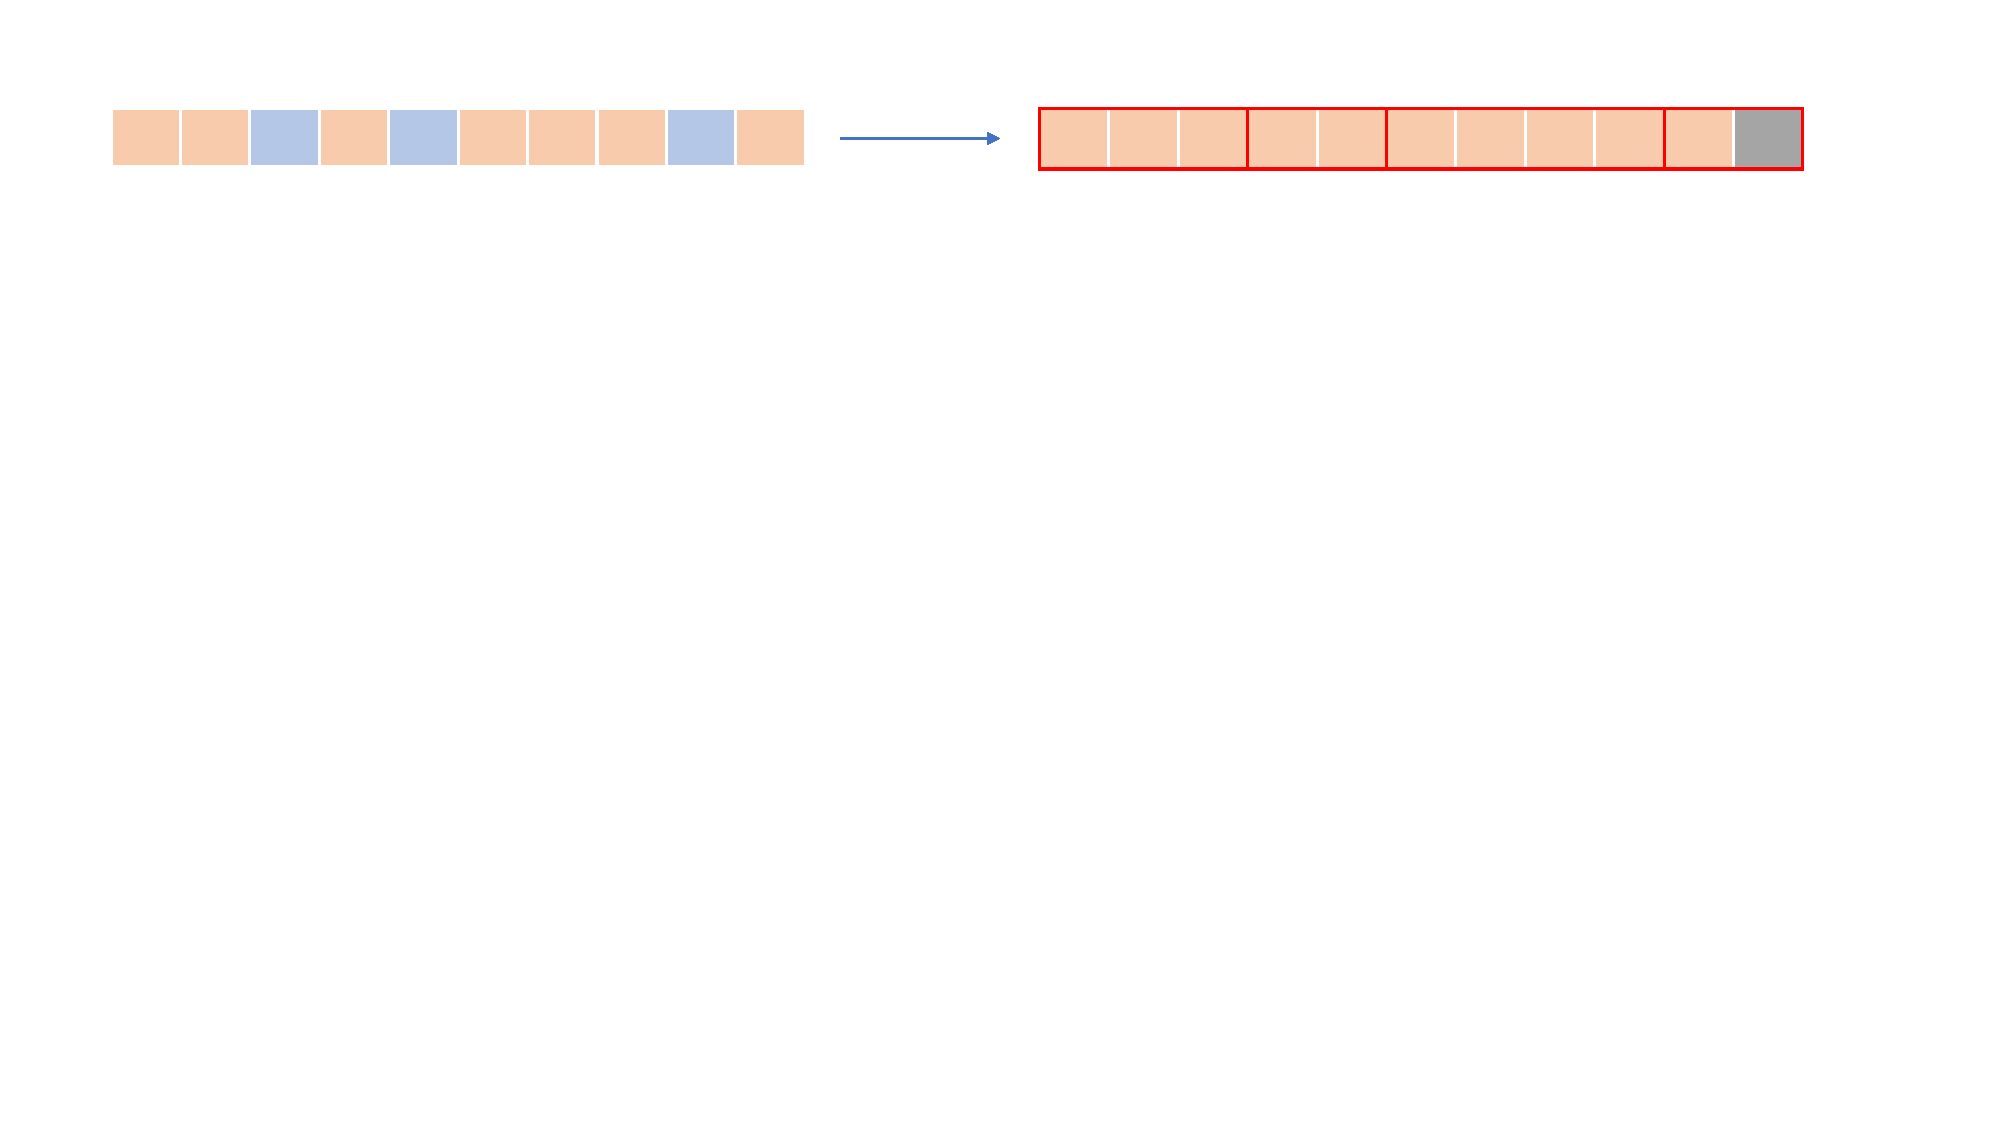
\includegraphics[width = 0.8\textwidth]{./Figures/dummy_seat.pdf}
%     \caption{Problem Conversion}
% \end{figure}

% The social distancing here is one seat. On the left side of the diagram, the blue squares represent the empty seats required for social distancing, while the orange squares represent the seats occupied by groups. On the right side, we have added one dummy seat at the end of each row. The orange squares surrounded by the red line represent the seats taken by groups in this row, which includes two groups of 1, one group of 2, and one group of 3.

% To represent a pattern with a fixed length of form, we can use a $(M+1)-$dimensional vector with $M$ group types. The aggregated form can be expressed as $[n_0, n_1, \ldots, n_M]$, where $n_i$ is the number of $i$-th group type, $i \in \mathcal{M}$. $n_0$ is the number of left seat, its value can only be $0, 1$ because two or more left seats will be assigned to groups. Thus the pattern, $[1, 0, 0, 0, 4]$, is not full because there is one left seat.


% \begin{prop}
% For the seat layout, $\{L_1, L_2, \ldots, L_{N}\}$, the minimal total loss is $\sum_{j} (\lfloor \frac{L_j}{n_{M}} \rfloor \delta -\delta + f(L_j \mod n_{M}))$. The maximal number of people assigned is $\sum_{j} (L_j - \lfloor \frac{L_j}{n_{M}} \rfloor - f(L_j \mod n_{M}))$.
% \end{prop}

\subsection{Dynamic Seat Assignment with Social Distancing}\label{sec_dynamic}
In a more realistic scenario, groups arrive dynamically, and the seller needs to make sequential decisions regarding group assignments while ensuring the required spacing between groups. When a group is accepted, the seller must also determine which seats should be assigned to that group. It is essential to note that each group must be either accepted in its entirety or rejected entirely; partial acceptance is not permitted. Once the seats are confirmed and assigned to a group, they cannot be changed or reassigned to other groups.

% We address the problem of dynamic seat assignment with social distancing, which involves the real-time allocation of seats to incoming groups while ensuring adherence to social distancing guidelines.
% We assume at most one arrival in each period, more than one arrival is negligible. 

To model this problem, we adopt a discrete-time framework. Time is divided into $T$ periods, indexed forward from $1$ to $T$. We assume that in each period, at most one group arrives and the probability of an arrival for a group of size $i$ is denoted as $p_i$, where $i$ belongs to the set $\mathcal{M}$. The probabilities satisfy the constraint $\sum_{i=1}^M p_i \leq 1$, indicating that the total probability of any group arriving in a single period does not exceed one. We introduce the probability $p_0 = 1 - \sum_{i=1}^{M} p_i$ to represent the probability of no arrival in a given period $t$. To simplify the analysis, we assume that the arrivals of different group types are independent and the arrival probabilities remain constant over time. This assumption can be extended to consider dependent arrival probabilities over time if necessary.

The state of remaining capacity in each row is represented by a vector $\mathbf{L} = (l_1, l_2, \ldots, l_N)$, where $l_j$ denotes the number of remaining seats in row $j$. Upon the arrival of a group type $i$ in period $t$, the seller needs to make a decision denoted by $u_{i,j}$, where $u_{i,j}(t) = 1$ indicates acceptance of group type $i$ in row $j$ during period $t$, while $u_{i,j}(t) = 0$ signifies rejection of that group type in row $j$ at that period. The feasible decision set is defined as $$U(\mathbf{L}) = \{u_{i,j} \in \{0,1\}, \forall i \in \mathcal{M}, \forall j \in \mathcal{N} | \sum_{j=1}^{N} u_{i,j} \leq 1, \forall i \in \mathcal{M}; n_{i}u_{i,j}\mathbf{e}_j \leq \mathbf{L}, \forall i \in \mathcal{M}, \forall j \in \mathcal{N}\}.$$ Here, $\mathbf{e}_j$ represents an N-dimensional unit column vector with the $j$-th element being 1, i.e., $\mathbf{e}_j = (\underbrace{0, \cdots, 0}_{j-1}, 1, \underbrace{0, \cdots, 0}_{n-j})$. In other words, the decision set $U(\mathbf{L})$ consists of all possible combinations of acceptance and rejection decisions for each group type in each row, subject to the constraints that at most one group of each type can be accepted in any row, and the number of seats occupied by each accepted group must not exceed the remaining capacity of the row.


Let $V_t(\mathbf{L})$ denote the maximum expected value to go, given remaining capacity $\mathbf{L}$ in period $t$. Then, the dynamic programming formula for this problem can be expressed as:

\begin{equation}\label{DP}
V_{t}(\mathbf{L}) = \max_{u_{i,j} \in U(\mathbf{L})}\left\{ \sum_{i=1}^{M} p_i ( \sum_{j=1}^{N} i u_{i,j} + V_{t+1}(\mathbf{L}- \sum_{j=1}^{N} n_i u_{i,j}\mathbf{e}_j)) + p_0 V_{t+1}(\mathbf{L})\right\}
\end{equation}

with the boundary conditions $V_{T+1}(\mathbf{L}) = 0, \forall \mathbf{L}, V_{t}(\mathbf{0}) =0, \forall t$.

At the beginning of period $t$, we have the current remaining capacity vector denoted as $\mathbf{L} = (L_1, L_2, \ldots, L_N)$. Our objective is to make decisions that maximize the total expected revenue during the selling horizon from period 1 to $T$. This maximum expected revenue is represented by $V_1(\mathbf{L})$, which captures the optimal value obtained by making the best decisions regarding group acceptance and seat assignments starting from the first period with the initial remaining capacity vector $\mathbf{L}$.

It is difficult to solve the DP \eqref{DP} due to the curse of dimensionality. To avoid this complexity, we seek to develop the heuristic method to assign arriving groups. It consists of generating the seat planning in Section 4 and stochastic assignment policy in Section 5.

% We propose an approach that directly targets the seat planning and then formulate a policy to assign arriving groups. To obtain the seat planning firstly, we develop the scenario-based stochastic programming.


% Our goal is to make the decision such as to maximize the total expected revenue in selling horizon from 1 to $T$, given by $V_1(\mathbf{L})$.

% Specifically, we define the concept of target seating plans deemed satisfactory. In making the dynamic seating plan, we will try to maintain the possibility of achieving one of the target seating plans as much as possible.